% !Mode:: "TeX:UTF-8:Main"

%needs currently a develepment version of expl3!
\documentclass{article}
\usepackage{l3draw}
\usepackage{tikzducks}
\begin{document}
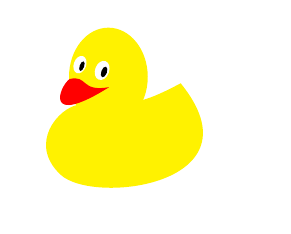
\begin{tikzpicture}
\fill[yellow](0.90,1.50) ellipse (0.50 and 0.625);

\fill[white, rotate=-20]
	(0.23,1.7675) ellipse (0.0893 and 0.125);
\fill[black, rotate=-20]
	(0.26,1.7575) ellipse (0.0357 and 0.0714);
\fill[white, rotate=-20]
	(-0.06,1.74) ellipse (0.0786 and 0.1143);
\fill[black, rotate=-20]
	(-0.03,1.73) ellipse (0.0286 and 0.0643);

\fill[red]	(0.406,1.472) .. controls (0.643,1.530) and (0.541,1.303) ..
	(0.910,1.370) .. controls (0.083,0.850) and (0.269,1.369) ..
	(0.406,1.472) -- cycle;

\fill[yellow] 	(0.513,1.145) .. controls (0.267, 1.102) and (-0.125,0.657) ..
  (0.289,0.261) .. controls (0.704,-0.135) and ( 2.863,0.130) ..
  (1.818,1.419) .. controls (0.938, 0.946) and ( 1.240,1.379) ..
  (0.513,1.145) -- cycle;
\end{tikzpicture}
%
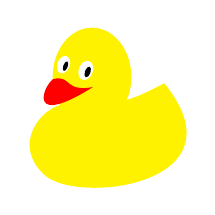
\begin{tikzpicture}
\duck[body=yellow,bill=red,eye=white,pupil=black]
\end{tikzpicture}
\ExplSyntaxOn
\draw_begin:
\driver_draw_fill_cmyk:nnnn {0} {0}{1}{0}
 %\draw_path_ellipse:nnn { 1cm , 0cm } { 1.5cm , 0cm } { 0cm , 1cm }
\draw_path_ellipse:nnn {0.90cm,1.50cm}  {0.5cm,0cm} {0cm,0.625cm}
\draw_path_use_clear:n { fill }

%body
\draw_path_moveto:n    {0.513cm,1.145cm}
%last argument: target point, before the control points. 
\draw_path_curveto:nnn {0.267cm, 1.102cm}{-0.125cm,0.657cm}{0.289cm,0.261cm}
\draw_path_curveto:nnn {0.704cm,-0.135cm}{2.863cm,0.130cm}{1.818cm,1.419cm}
\draw_path_curveto:nnn {0.938cm, 0.946cm}{1.240cm,1.379cm}{0.513cm,1.145cm}
\draw_path_close: %needed?
\draw_path_use_clear:n { fill }

%bill
\driver_draw_fill_rgb:nnn {1} {0}{0}
\draw_path_moveto:n    {0.406cm,1.472cm}
\draw_path_curveto:nnn {0.643cm,1.530cm}{0.541cm,1.303cm}{0.910cm,1.370cm}
\draw_path_curveto:nnn {0.083cm,0.850cm}{0.269cm,1.369cm}{0.406cm,1.472cm}
\draw_path_close: %needed?
\draw_path_use_clear:n { fill }

%rotate -20: 
%\driver_draw_transformcm:nnnnnn
% {\fp_eval:n{cosd(20)}} {\fp_eval:n{-sind(20)}}
% {\fp_eval:n{sind(20)}} {\fp_eval:n{cosd(20)}}
% {0cm}{0cm}
\draw_transform:nnnnn
 {cosd(20)} {-sind(20)}
 {sind(20)} {cosd(20)} { 0cm , 0cm }
 
%eyes 
\driver_draw_fill_cmyk:nnnn {0}{0}{0}{0} 
\draw_path_ellipse:nnn {0.23cm,1.7675cm}  {0.0893cm,0cm} {0cm,0.125cm}
\draw_path_use_clear:n { fill }

\draw_path_ellipse:nnn {-0.06cm,1.74cm}  {0.0786cm,0cm} {0cm,0.1143cm}
\draw_path_use_clear:n { fill }

%pupils
\driver_draw_fill_cmyk:nnnn {0}{0}{0}{1}
\draw_path_ellipse:nnn {0.26cm,1.7575cm}  {0.0357cm,0cm} {0cm,0.0714cm}
\draw_path_use_clear:n { fill }

\draw_path_ellipse:nnn {-0.03cm,1.73cm}  {0.0286cm,0cm} {0cm,0.0643cm}
\draw_path_use_clear:n { fill }

\draw_end:
\par


%again but now without cm as unit
\newcommand\myduck[1]{
\draw_begin:
\draw_transform:nnnnn { #1 } { 0 } { 0 } { #1 } { 0 , 0 }

\driver_draw_fill_cmyk:nnnn {0} {0}{1}{0}
\draw_path_ellipse:nnn {0.90,1.50}  {0.5,0} {0,0.625}
 \draw_path_use_clear:n { fill }

%body
\draw_path_moveto:n    {0.513,1.145}
%last argument: target point, before the control points.
\draw_path_curveto:nnn {0.267, 1.102}{-0.125,0.657}{0.289,0.261}
\draw_path_curveto:nnn {0.704,-0.135}{2.863,0.130}{1.818,1.419}
\draw_path_curveto:nnn {0.938, 0.946}{1.240,1.379}{0.513,1.145}
\draw_path_close: %needed?
 \draw_path_use_clear:n { fill }

%bill
\driver_draw_fill_rgb:nnn {1} {0}{0}
\draw_path_moveto:n    {0.406,1.472}
\draw_path_curveto:nnn {0.643,1.530}{0.541,1.303}{0.910,1.370}
\draw_path_curveto:nnn {0.083,0.850}{0.269,1.369}{0.406,1.472}
\draw_path_close: %needed?
\draw_path_use_clear:n { fill }

\draw_transform_concat:nnnnn
 {cosd(20)} {-sind(20)}
 {sind(20)} {cosd(20)} { 0 , 0 }
 
%eyes
\driver_draw_fill_cmyk:nnnn {0}{0}{0}{0}
\draw_path_ellipse:nnn {0.23,1.7675}  {0.0893,0} {0,0.125}
\draw_path_use_clear:n { fill }

\draw_path_ellipse:nnn {-0.06,1.74}  {0.0786,0} {0,0.1143}
\draw_path_use_clear:n { fill }

%pupils
\driver_draw_fill_cmyk:nnnn {0}{0}{0}{1}
\draw_path_ellipse:nnn {0.26,1.7575}  {0.0357,0} {0,0.0714}
\draw_path_use_clear:n { fill }

\draw_path_ellipse:nnn {-0.03,1.73}  {0.0286,0} {0,0.0643}
\draw_path_use_clear:n { fill }

\draw_end:}

\bigskip
\myduck{1cm} \myduck{0.8cm} \myduck{0.6cm} 
\ExplSyntaxOff

\end{document} 